\chapter{电池、燃料电池与电解}\label{ch:b2:batteries-electrolysis}

每千克从矿石中提取的铝约需 \qty{13}{kW.h} 的
电能；若将一千克废铝重新熔化，理论上只需
\qty{0.3}{kW.h} 即可将其加热至熔点并使之熔化。两者之差
即一长排\omterm{def:b2:batteries-electrolysis:electrolysis}{电解槽}所做的功，每个\omterm{def:b2:batteries-electrolysis:electrolysis}{电解槽}在熔盐中通过
数十万安培的电流，电压仅为几伏。电池则恰好相反：
由自发反应驱动电流。借助
\cref{ch:b2:current-potential-curves}中的\omterm{def:b2:current-potential-curves:ie-curve}{电流–电势曲线}，
两者以及锌片在酸中的溶解，都可在同一张图上读出。
% ledger: hT:Al_l.933, aw:Al

\begin{recall}
由\cref{ch:b2:cell-thermodynamics}可知：$\Delta_r G = -nFE$，即最大功，以及
\omterm{def:b2:cell-thermodynamics:faraday}{法拉第常数}。由\cref{ch:b2:current-potential-curves}可知：\omterm{def:b2:current-potential-curves:ie-curve}{电流–电势曲线}、
\omterm{def:b2:current-potential-curves:fast-slow}{快速体系}与\omterm{def:b2:current-potential-curves:fast-slow}{慢速体系}、\omterm{def:b2:current-potential-curves:overpotential}{过电势}、\omterm{def:b2:current-potential-curves:limiting-current}{极限电流}，以及
水的分解界限。由\cref{ch:b2:ellingham}可知：为何不能用碳还原获得铝。
第 1 册：\omterm{def:b2:batteries-electrolysis:electrolysis}{电解}、\omterm{def:b2:batteries-electrolysis:battery}{蓄电池}。
\end{recall}

\begin{omfigure}
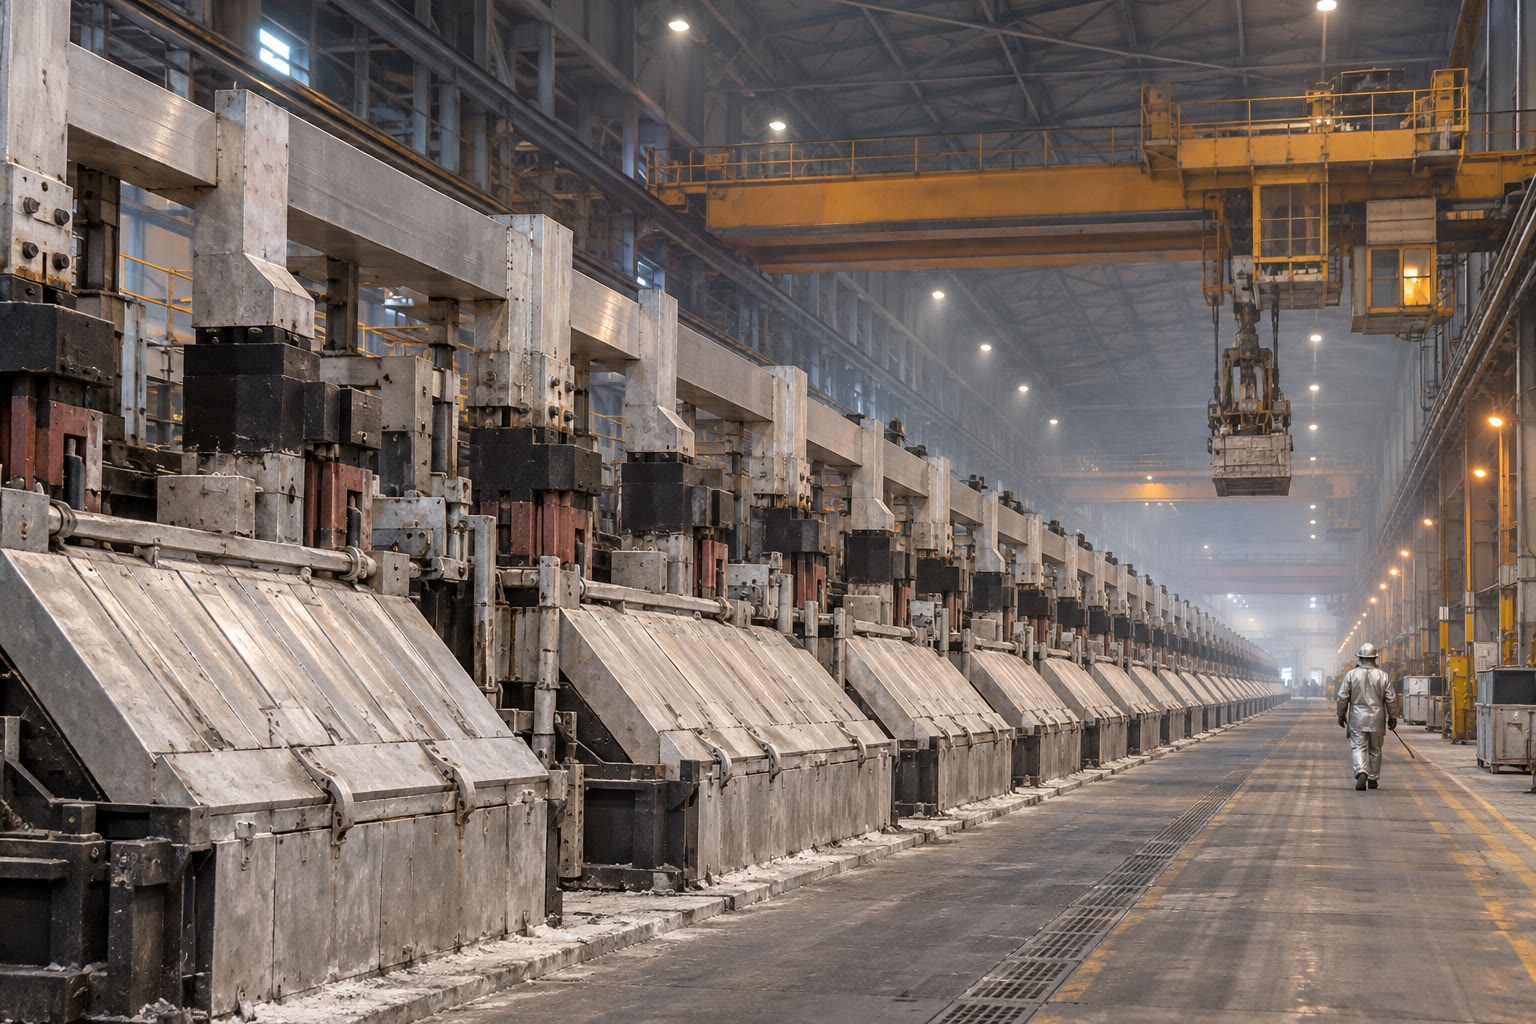
\includegraphics[width=0.62\linewidth]{images/book3/ai/b2-11-potroom.jpg}

{\small 铝\omterm{def:b2:batteries-electrolysis:electrolysis}{电解}厂的\omterm{def:b2:batteries-electrolysis:electrolysis}{电解}车间：一排\omterm{def:b2:batteries-electrolysis:electrolysis}{电解槽}，
长达数百个，彼此串联；车间上方的吊车
更换逐渐烧损的碳阳极。}
\end{omfigure}

\section{在曲线上读取自发反应}

\begin{definition}[混合电势]\label{def:b2:batteries-electrolysis:mixed-potential}
若电极上两种不同电对发生反应，一者被氧化、一者被还原，则称该电极的\emph{混合电势}\index{混合电势}
为净电流为零时电极所具有的电势，此时
一个电对的\omterm{def:b2:current-potential-curves:ie-curve}{阳极电流}与另一电对的\omterm{def:b2:current-potential-curves:ie-curve}{阴极电流}
大小相等、方向相反。
\end{definition}

\begin{proposition}[金属在溶液中]\label{prop:b2:batteries-electrolysis:mixed}
金属浸入能将其氧化的溶液中时，稳定于电势
$E_m$，满足 $i_a(E_m) = -i_c(E_m)$，即金属氧化的\omterm{def:b2:current-potential-curves:ie-curve}{阳极电流}
与氧化剂还原的\omterm{def:b2:current-potential-curves:ie-curve}{阴极电流}相互平衡；金属的溶解速率
为 $i_a(E_m)/(nF)$。
\end{proposition}

\begin{proof}
孤立的金属片上没有净电流。两个半反应
同时在其表面、相同电势下发生，因此在该电势下读取的电流
两者之和为零。由\cref{prop:b2:current-potential-curves:current-rate}可知，
\omterm{def:b2:current-potential-curves:ie-curve}{阳极电流}即给出氧化速率。
\end{proof}

\begin{omfigure}
\begin{tikzpicture}
\begin{axis}[omie, width=0.82\linewidth, height=6cm, xmin=-1.1, xmax=-0.3,
  ymin=-3, ymax=3, xlabel={$E$ (V)}, ylabel={$i$}, clip=true, clip mode=individual,
  axis y line=left]
\addplot[omanodic] table[x=E, y=i] {figdata/out/bachelor-2-ie-curves-f-Zn.dat};
\addplot[omcathodic] table[x=E, y=i] {figdata/out/bachelor-2-ie-curves-f-HZn.dat};
\addplot[omcathodic, dashed] table[x=E, y=i] {figdata/out/bachelor-2-ie-curves-f-HCu.dat};
\draw[densely dotted] (axis cs:-0.820,-0.148) -- (axis cs:-0.820,0.148);
\draw[densely dotted] (axis cs:-0.737,-2.38) -- (axis cs:-0.737,2.38);
\fill (axis cs:-0.820,0.148) circle (1.3pt); \fill (axis cs:-0.737,2.38) circle (1.3pt);
\node[font=\scriptsize, anchor=south east] at (axis cs:-0.825,0.2) {锌单独存在};
\node[font=\scriptsize, anchor=west] at (axis cs:-0.73,2.38) {锌与铜接触};
\node[font=\scriptsize, omThm, anchor=west] at (axis cs:-0.70,1.2) {\ce{Zn} $\to$ \ce{Zn^2+}};
\node[font=\scriptsize, omDef, anchor=north west, align=left] at (axis cs:-0.87,-0.5) {\ce{H+} $\to$ \ce{H2}\\ 在锌上};
\node[font=\scriptsize, omDef, anchor=north west] at (axis cs:-0.66,-1.7) {在铜上};
\end{axis}
\end{tikzpicture}

{\small 锌在酸中（模型曲线，锌离子浓度较低；电势从
$-1.1$ 到 \qty{-0.3}{V}）。锌单独存在时，其电势
稳定于\omterm{def:b2:batteries-electrolysis:mixed-potential}{混合电势}，此时锌的氧化与
\ce{H+} 在锌上的缓慢还原相互平衡：电流很小，溶解缓慢。与铜接触时，
\ce{H+} 在铜上的还原不那么缓慢，平衡移向更高的电势，
电流比前者大十倍以上：锌迅速溶解，氢气
在铜上冒出气泡。}
\end{omfigure}

同一读图方法也可解释腐蚀（见\cref{ch:b2:corrosion}）：金属的
腐蚀速率即为其在\omterm{def:b2:batteries-electrolysis:mixed-potential}{混合电势}下的电流。

\section{输出电流的电池}

\begin{definition}[电池]\label{def:b2:batteries-electrolysis:battery}
\emph{一次电池}\index{一次电池}是仅使用一次的电化学电池，
即用至反应物耗尽为止。\emph{蓄电池}\index{蓄电池}是
可通过反向通入电流而充电的电池，
充电会使其反应逆转。电池的\emph{比能量}\index{比能量}
是指单位质量所输出的电能，
通常以 \unit{W.h/kg} 表示。
\end{definition}

\begin{proposition}[输出电流时电池的电压]\label{prop:b2:batteries-electrolysis:delivering}
输出电流 $I$ 的电池，其电压为
\[
  U = E_+ - E_- - \eta_a - |\eta_c| - rI ,
\]
其中 $E_+$ 与 $E_-$ 为其两个电极的平衡电势，
$\eta_a > 0$ 为负极上氧化的\omterm{def:b2:current-potential-curves:overpotential}{过电势}，
$\eta_c < 0$ 为正极上还原的\omterm{def:b2:current-potential-curves:overpotential}{过电势}，$r$ 为
内阻（包括\omterm{def:b2:batteries-electrolysis:electrolysis}{电解}质、隔膜与连接部分）。
\end{proposition}

\begin{proof}
同一电流 $I$ 在负极上为\omterm{def:b2:current-potential-curves:ie-curve}{阳极电流}，其电势
由其阳极曲线读取，为 $E_- + \eta_a$；在正极上则为\omterm{def:b2:current-potential-curves:ie-curve}{阴极电流}，
电势为 $E_+ + \eta_c$。电流穿过二者之间的
\omterm{def:b2:batteries-electrolysis:electrolysis}{电解}质，电势降低 $rI$。由此得 $U = (E_+ + \eta_c) - (E_- +
\eta_a) - rI$。
\end{proof}

\begin{omfigure}
\begin{tikzpicture}
\begin{axis}[omie, width=0.82\linewidth, height=5.6cm, xmin=-1.2, xmax=0.8,
  ymin=-2, ymax=2, xlabel={$E$ (V)}, ylabel={$i$}, clip=true, clip mode=individual]
\addplot[omanodic] table[x=E, y=i] {figdata/out/bachelor-2-ie-curves-h-neg.dat};
\addplot[omcathodic] table[x=E, y=i] {figdata/out/bachelor-2-ie-curves-h-pos.dat};
\draw[densely dashed, gray] (axis cs:-1.2,1) -- (axis cs:0.8,1);
\draw[densely dashed, gray] (axis cs:-1.2,-1) -- (axis cs:0.8,-1);
\node[font=\scriptsize, gray, anchor=south west] at (axis cs:-1.18,1) {$+I$};
\node[font=\scriptsize, gray, anchor=north west] at (axis cs:-1.18,-1) {$-I$};
\fill (axis cs:-0.730,1) circle (1.3pt); \fill (axis cs:0.210,-1) circle (1.3pt);
\draw[densely dotted] (axis cs:-0.85,0) -- (axis cs:-0.85,0.5);
\draw[densely dotted] (axis cs:0.45,0) -- (axis cs:0.45,-0.5);
\node[font=\scriptsize, anchor=south] at (axis cs:-0.85,0.5) {$E_-$};
\node[font=\scriptsize, anchor=north] at (axis cs:0.45,-0.5) {$E_+$};
\draw[<->, thick, omProp] (axis cs:-0.730,1.5) -- (axis cs:0.210,1.5) node[midway, above, font=\scriptsize] {$U + rI$};
\draw[densely dotted] (axis cs:-0.730,1) -- (axis cs:-0.730,1.5);
\draw[densely dotted] (axis cs:0.210,-1) -- (axis cs:0.210,1.5);
\node[font=\scriptsize, omThm, anchor=west] at (axis cs:-0.70,0.6) {负极};
\node[font=\scriptsize, omDef, anchor=west] at (axis cs:0.30,-1.5) {正极};
\end{axis}
\end{tikzpicture}

{\small 电池的工作点（模型曲线）。在电流 $I$ 下，负极
位于其阳极曲线上，正极位于其阴极曲线上；两极电势之差，
减去欧姆降 $rI$，即为输出电压。
它随 $I$ 增大而下降。}
\end{omfigure}

\begin{method}[电池或电解槽的工作点]\label{met:b2:batteries-electrolysis:operating-point}
\begin{enumerate}
  \item 画出被氧化的电极的阳极曲线，以及
        被还原的电极的阴极曲线。
  \item 对于电流 $I$，读取各电极的电势：在 $+I$ 处取阳极曲线上的值，
        在 $-I$ 处取阴极曲线上的值。
  \item 两极电势之差经 $rI$ 修正（电池中减去，
        \omterm{def:b2:batteries-electrolysis:electrolysis}{电解槽}中加上），即为电压。
\end{enumerate}
\end{method}

\begin{example}[铅酸蓄电池]\label{ex:b2:batteries-electrolysis:lead}
负极上 \ce{Pb + SO4^2- -> PbSO4 + 2e-}；正极上
为 \ce{PbO2 + 4H+ + SO4^2- + 2e- -> PbSO4 + 2H2O}。总反应为
\[
  \ce{Pb + PbO2 + 4H+ + 2SO4^2- -> 2PbSO4 + 2H2O},
\]
$\Delta_r G^\circ = 2(-813.14) + 2(-237.13) - (-217.33) - 2(-744.53) =
\qty{-394.1}{kJ/mol}$, $E^\circ = 394\,100/(2 \times 96\,485) = \qty{2.04}{V}$.
放电时两极均被硫酸铅覆盖，充电则
使反应逆转。铅上 \ce{H+} 的还原与二氧化铅上
水的氧化都很慢，这正是 \qty{2}{V} 的电池能在
水中充电的原因，水的热力学窗口宽度仅为 \qty{1.23}{V}。
% ledger: dfg:PbSO4_cr, dfg:H2O_l, dfg:PbO2_cr, dfg:SO42-_ao
\end{example}

\begin{omfigure}
\begin{tikzpicture}[font=\small, >={Stealth}]
  \draw[thick] (0,0) rectangle (6,3.2);
  \fill[omDef!10] (0.05,0.05) rectangle (5.95,2.7);
  \fill[black!45] (0.6,0.4) rectangle (1.1,2.9);
  \fill[brown!60!black] (4.9,0.4) rectangle (5.4,2.9);
  \draw[thick] (0.85,2.9) -- (0.85,3.9) node[pos=0.75, left] {$-$};
  \draw[thick] (5.15,2.9) -- (5.15,3.9) node[pos=0.75, right] {$+$};
  \draw[->, thick, omProp] (0.85,3.9) -- (0.85,4.3) -- (5.15,4.3) -- (5.15,3.95);
  \node[font=\scriptsize, omProp, anchor=south] at (3,4.3) {放电时 $\mathrm{e^-}$};
  \node[font=\scriptsize, align=center] at (0.85,-0.45) {\ce{Pb}\\ （放电时为 \ce{PbSO4}）};
  \node[font=\scriptsize, align=center] at (5.15,-0.45) {\ce{PbO2}\\ （放电时为 \ce{PbSO4}）};
  \node[font=\scriptsize, align=center] at (3.0,1.6) {\ce{H2SO4} 溶液 \\ \ce{H+}、\ce{HSO4-}、\ce{SO4^2-}};
\end{tikzpicture}

{\small 铅酸\omterm{def:b2:batteries-electrolysis:battery}{蓄电池}示意图。放电时，铅被氧化，
二者均被还原为硫酸铅，硫酸被消耗：
溶液的密度可指示充电状态。}
\end{omfigure}

\begin{omfigure}
\begin{tikzpicture}[font=\small, >={Stealth}]
  \draw[thick] (0,0) rectangle (7,3);
  % graphite layers
  \foreach \y in {0.5,0.9,1.3,1.7,2.1,2.5} \draw[thick, black!70] (0.3,\y) -- (2.3,\y);
  \foreach \y in {0.7,1.1,1.5,1.9,2.3} \foreach \x in {0.6,1.3,2.0} \fill[omDef] (\x,\y) circle (0.07);
  % layered oxide
  \foreach \y in {0.5,0.9,1.3,1.7,2.1,2.5} \draw[thick, omThm] (4.7,\y) -- (6.7,\y);
  \foreach \y in {0.7,1.5,2.3} \foreach \x in {5.0,5.7,6.4} \fill[omDef] (\x,\y) circle (0.07);
  \draw[densely dashed] (3.5,0) -- (3.5,3);
  \node[font=\scriptsize, align=center] at (1.3,-0.45) {石墨（负极）};
  \node[font=\scriptsize, align=center] at (5.7,-0.45) {层状氧化物（正极）};
  \node[font=\scriptsize, anchor=south] at (3.5,3.0) {隔膜};
  \draw[->, thick, omThm] (2.5,2.1) -- (4.5,2.1) node[midway, above, font=\scriptsize, fill=white, inner sep=1pt] {\ce{Li+} 放电时};
  \draw[<-, thick, omDef] (2.5,0.9) -- (4.5,0.9) node[midway, below, font=\scriptsize, fill=white, inner sep=1pt] {\ce{Li+} 充电时};
\end{tikzpicture}

{\small 锂离子电池示意图。锂离子（蓝点）位于充电后的电池中
石墨层之间；放电时，它们穿过
\omterm{def:b2:batteries-electrolysis:electrolysis}{电解}质，嵌入金属氧化物的层间，同时电子经外电路流动，
两极既不溶解也不沉积：
离子在两种宿主之间往返穿梭。}
\end{omfigure}

\begin{history}[伏打电堆]
\begin{minipage}[t]{0.27\linewidth}
\vspace{0pt}
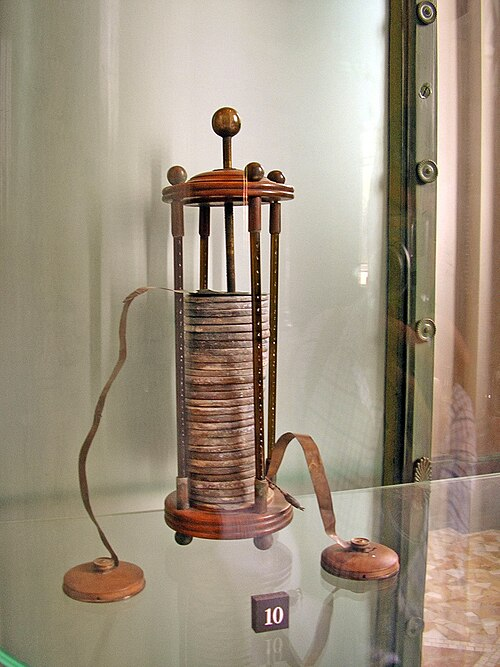
\includegraphics[width=\linewidth]{images/book3/volta-pile.jpg}
\end{minipage}\hfill
\begin{minipage}[t]{0.69\linewidth}
\vspace{0pt}
1800 年，亚历山德罗·伏打描述了一根由两种不同金属圆片叠成的柱，
圆片分别为锌与铜或银，中间以浸过盐水的布隔开：这是第一个
能提供稳定电流的电源。数周之内，他人便用它分解水；
十年之内，汉弗莱·戴维用大型电堆，
\omterm{def:b2:batteries-electrolysis:electrolysis}{电解}其熔融氢氧化物，分离出钠和钾。照片所示为
伏打本人所制电堆之一。（照片：GuidoB，CC BY-SA 3.0，维基共享资源
。）
\end{minipage}
\end{history}

\section{燃料电池}

\begin{definition}[燃料电池]\label{def:b2:batteries-electrolysis:fuel-cell}
称\emph{燃料电池}\index{燃料电池}为这样一种电池：其反应物（燃料与氧化剂，通常为空气中的氧）
被连续输入其电极，其产物被不断移出，
从而只要持续供给，
它便持续输出电流。
\end{definition}

在公交车所用的质子交换膜电池中（见
\cref{ch:b2:cell-thermodynamics}），氢在铂催化剂上被氧化，
\ce{H2 -> 2H+ + 2e-}，质子穿过一层薄的酸性聚合物膜，
氧在另一侧被还原，\ce{O2 + 4H+ + 4e- -> 2H2O}。氢的氧化
在铂上进行，属\omterm{def:b2:current-potential-curves:fast-slow}{快速体系}；氧的还原在各电极上都很慢。
可逆电池的 \qty{1.23}{V} 与工作电压之间损失的电压中，
大部分为氧电极的\omterm{def:b2:current-potential-curves:overpotential}{过电势}，
其余为膜的电阻，以及大电流下氧向催化剂的供应，
后者即（为一种）\omterm{def:b2:current-potential-curves:limiting-current}{极限电流}。

\section{电解}

\begin{definition}[电解]\label{def:b2:batteries-electrolysis:electrolysis}
称\emph{电解}\index{电解}为一种非自发的氧化还原反应，
由外接发电机提供的电流所驱动；发生该反应的电池称为
\emph{电解槽}\index{电解槽}。阳极是发生氧化的一极，
与发电机的正极相连。
\end{definition}

\begin{proposition}[热力学最小电压]\label{prop:b2:batteries-electrolysis:minimum-voltage}
\omterm{def:b2:batteries-electrolysis:electrolysis}{电解}反应满足 $\Delta_r G > 0$ 时，
所需电压至少为 $\Delta_r G/(nF)$。
\end{proposition}

\begin{proof}
发电机每摩尔反应提供的功为 $nFU$；
对逆反应应用\cref{thm:b2:cell-thermodynamics:delta-g-nfe}，
所接收的电功至少为 $\Delta_r G$。
\end{proof}

\begin{proposition}[电解槽的电压]\label{prop:b2:batteries-electrolysis:electrolysis-voltage}
通过电流 $I$ 的\omterm{def:b2:batteries-electrolysis:electrolysis}{电解槽}所需电压为
\[
  U = (E_a - E_c) + \eta_a + |\eta_c| + rI ,
\]
其中 $E_a$、$E_c$ 分别为阳极与阴极电对的平衡电势，
（$E_a - E_c = \Delta_r G/(nF)$），$\eta_a$、$\eta_c$ 为该电流下的\omterm{def:b2:current-potential-curves:overpotential}{过电势}，
以及 $r$ 为两电极之间的电阻。
\end{proposition}

\begin{proof}
与电池情形相同，同一电流在阳极处为\omterm{def:b2:current-potential-curves:ie-curve}{阳极电流}，电势为 $E_a +
\eta_a$；在阴极处为\omterm{def:b2:current-potential-curves:ie-curve}{阴极电流}，电势为 $E_c + \eta_c$；发电机还必须
另需驱动电流通过\omterm{def:b2:batteries-electrolysis:electrolysis}{电解}质，增加 $rI$。
\end{proof}

\begin{method}[预测电解过程]\label{met:b2:batteries-electrolysis:predict-electrolysis}
\begin{enumerate}
  \item 列出所有可能在阳极被氧化的物种（包括阳极金属
        与溶剂），以及所有可能在阴极被还原的物种
        （包括溶剂）。
  \item 在所用电极材料上画出它们的\omterm{def:b2:current-potential-curves:ie-curve}{电流–电势曲线}。
  \item 随着电压升高，最先到达的\omterm{def:b2:current-potential-curves:ie-curve}{阳极电流}曲线与最先到达的
        \omterm{def:b2:current-potential-curves:ie-curve}{阴极电流}曲线给出相应反应；电流更大时，后续曲线
        各自加入其反应。
\end{enumerate}
\end{method}

\begin{definition}[法拉第效率]\label{def:b2:batteries-electrolysis:faradaic-efficiency}
称\omterm{def:b2:batteries-electrolysis:electrolysis}{电解}的\emph{法拉第效率}\index{法拉第效率} $\eta_F$ 为
通过的电量中生成目标产物的那部分所占的分数。
其\emph{比能耗}\index{比能耗}为
即生成单位质量产物所消耗的电能。
\end{definition}

\begin{proposition}[法拉第电磁感应定律]\label{prop:b2:batteries-electrolysis:faraday-mass}
电流 $I$ 通过时间 $t$、\omterm{def:b2:batteries-electrolysis:faradaic-efficiency}{法拉第效率}为 $\eta_F$ 时，
生成质量为 $m = \eta_F MIt/(nF)$ 的产物，该产物的摩尔质量为 $M$，
每生成一摩尔产物转移 $n$ 个电子。
\end{proposition}

\begin{proof}
电荷 $It$ 中有 $\eta_F It$ 用于生成产物，
由\cref{prop:b2:cell-thermodynamics:charge}可知其对应 $\eta_F It/(nF)$ 摩尔。
\end{proof}

\begin{proposition}[每千克能耗]\label{prop:b2:batteries-electrolysis:energy}
在电压 $U$ 与\omterm{def:b2:batteries-electrolysis:faradaic-efficiency}{法拉第效率} $\eta_F$ 下，其\omterm{def:b2:batteries-electrolysis:faradaic-efficiency}{比能耗}
为 $w = nFU/(\eta_F M)$。
\end{proposition}

\begin{proof}
能量为 $UIt$，质量为 $\eta_F MIt/(nF)$，相除即得。
\end{proof}

\section{工业电解}

\paragraph{锌。} 大部分锌通过\omterm{def:b2:batteries-electrolysis:electrolysis}{电解}酸性硫酸锌
溶液制得（见\cref{ch:b2:ellingham}）。锌在阴极析出，尽管
\ce{H+} 是更强的氧化剂：在锌上 \ce{H+} 的还原很慢，
而锌的波先被达到；阳极放出氧气。

\begin{omfigure}
\begin{tikzpicture}
\begin{axis}[omie, width=0.82\linewidth, height=5.6cm, xmin=-1.6, xmax=2.4,
  ymin=-2.4, ymax=2.4, xlabel={$E$ (V)}, ylabel={$i$}, clip=true, clip mode=individual]
\addplot[omcathodic] table[x=E, y=i] {figdata/out/bachelor-2-ie-curves-g-cath.dat};
\addplot[omanodic] table[x=E, y=i] {figdata/out/bachelor-2-ie-curves-g-an.dat};
\draw[densely dotted] (axis cs:-0.76,-2.2) -- (axis cs:-0.76,0.4);
\draw[densely dotted] (axis cs:0,-2.2) -- (axis cs:0,0.4);
\node[font=\scriptsize, anchor=south] at (axis cs:-0.76,0.4) {$-0.76$};
\node[font=\scriptsize, anchor=south east] at (axis cs:-0.02,0.4) {$0$};
\node[font=\scriptsize, omDef, anchor=north west, align=left] at (axis cs:-0.7,-1.05) {\ce{Zn^2+} $\to$ \ce{Zn},\\ 平台};
\node[font=\scriptsize, omDef, anchor=east, align=right] at (axis cs:-1.32,-0.9) {\ce{H+} $\to$ \ce{H2}\\ 在锌上};
\node[font=\scriptsize, omThm, anchor=east] at (axis cs:1.85,1.6) {\ce{H2O} $\to$ \ce{O2}};
\node[font=\scriptsize, gray, align=center] at (axis cs:-0.38,-0.5) {\ce{H2}\\ 锌上此处无};
\end{axis}
\end{tikzpicture}

{\small 以锌为阴极\omterm{def:b2:batteries-electrolysis:electrolysis}{电解}酸性硫酸锌溶液
（模型曲线）。虽然 \ce{H+}/\ce{H2} 电对（$\qty{0}{V}$）
的电势高于 \ce{Zn^2+}/\ce{Zn} 电对（$\qty{-0.76}{V}$），
但 \ce{H+} 在锌上的还原要到约 \qty{-1.1}{V} 才开始，两者之间只沉积出锌。
阳极上水被氧化为氧气。}
\end{omfigure}

\paragraph{氯气与氢氧化钠。}盐水在一个\omterm{def:b2:batteries-electrolysis:electrolysis}{电解}池中\omterm{def:b2:batteries-electrolysis:electrolysis}{电解}，
该\omterm{def:b2:batteries-electrolysis:electrolysis}{电解}池由只允许阳离子通过的膜隔开。阳极上氯离子被
氧化：\ce{2Cl- -> Cl2 + 2e-}；阴极上水被还原：\ce{2H2O +
2e- -> H2 + 2OH-}；钠离子穿过膜以平衡电荷，
阴极一侧流出的是不含氯离子的氢氧化钠溶液。
热力学最小值为 $\Delta_r G/(2F) = \qty{2.19}{V}$，对应反应 \ce{2Cl- + 2H2O -> Cl2 +
H2 + 2OH-}（标准条件下）。氯气在阳极生成，而不是
氧气，尽管 \ce{O2}/\ce{H2O} 电对的电势更低：
在所用阳极材料上，水的氧化是两者中较慢的一个。
% ledger: dfg:OH-_ao, dfg:Cl-_ao, dfg:H2O_l

\begin{omfigure}
\begin{tikzpicture}[font=\small, >={Stealth}]
  \draw[thick] (0,0) rectangle (6,3.4);
  \draw[thick, dashed, omProp] (3,0) -- (3,3.4);
  \fill[black!30] (0.4,0.3) rectangle (0.7,3.0);
  \fill[black!50] (5.3,0.3) rectangle (5.6,3.0);
  \node[font=\scriptsize] at (0.55,3.3) {$+$};
  \node[font=\scriptsize] at (5.45,3.3) {$-$};
  \node[font=\scriptsize, align=center] at (1.85,1.9) {盐水 \\ \ce{2Cl-} $\to$\\ \ce{Cl2 + 2e-}};
  \node[font=\scriptsize, align=center] at (4.2,1.9) {\ce{NaOH}溶液 \\ \ce{2H2O + 2e-} $\to$\\ \ce{H2 + 2OH-}};
  \draw[->, thick, omDef] (2.6,0.8) -- (3.4,0.8) node[pos=0.1, above, font=\scriptsize] {\ce{Na+}};
  \draw[->, thick] (1.0,3.4) -- (1.0,4.0) node[above] {\ce{Cl2}};
  \draw[->, thick] (5.0,3.4) -- (5.0,4.0) node[above] {\ce{H2}};
  \draw[->, thick] (-0.8,0.6) -- (0,0.6) node[pos=0, left] {盐水进};
  \draw[->, thick] (6,0.6) -- (6.8,0.6) node[right] {\ce{NaOH} 出};
  \node[font=\scriptsize, omProp, anchor=north] at (3,-0.05) {阳离子交换膜};
\end{tikzpicture}

{\small 隔膜式氯碱\omterm{def:b2:batteries-electrolysis:electrolysis}{电解}池示意图。只有钠离子穿过
隔膜，因此阴极生成的氢氧化物不会与氯气接触。}
\end{omfigure}

\paragraph{铝。}氧化铝溶于熔融的冰晶石，
\ce{Na3AlF6}，其熔点远低于氧化铝，在
碳阴极（液态铝在其上聚集）与碳阳极之间\omterm{def:b2:batteries-electrolysis:electrolysis}{电解}，碳阳极
以二氧化碳形式烧掉（霍尔–埃鲁法）：
\[
  \ce{2Al2O3 + 3C -> 4Al + 3CO2} .
\]
在 \qty{1250}{K} 附近，热力学最小电压约为 \qty{1.18}{V}
（见\cref{pb:b2:batteries-electrolysis:1}）；该题中的\omterm{def:b2:batteries-electrolysis:electrolysis}{电解}池
工作电压为此值的三倍半，多出的部分转化为维持熔池
熔融的热量。

\begin{omfigure}
\begin{tikzpicture}[font=\small, >={Stealth}]
  \draw[thick, fill=black!12] (0,0) rectangle (7,3.2);
  \fill[black!45] (0.3,0.3) rectangle (6.7,0.8);
  \fill[gray!35] (0.3,0.8) rectangle (6.7,1.4);
  \fill[orange!30] (0.3,1.4) rectangle (6.7,2.5);
  \foreach \x in {1.0,3.0,5.0} {
    \fill[black!75] (\x,1.75) rectangle (\x+1.0,3.6);
    \draw[thick] (\x+0.5,3.6) -- (\x+0.5,4.2);
  }
  \draw[thick] (1.5,4.2) -- (5.5,4.2) node[right] {$+$};
  \node[font=\scriptsize, align=left, anchor=west] at (7.3,2.6) {碳阳极，烧成 \ce{CO2}};
  \node[font=\scriptsize, align=left, anchor=west] at (7.3,1.95) {熔融冰晶石 + 溶解的 \ce{Al2O3}};
  \node[font=\scriptsize, align=left, anchor=west] at (7.3,1.1) {液态铝（阴极）};
  \node[font=\scriptsize, align=left, anchor=west] at (7.3,0.55) {碳阴极块，$-$};
  \draw[densely dotted] (6.7,2.6) -- (7.3,2.6) (6.7,1.95) -- (7.3,1.95) (6.7,1.1) -- (7.3,1.1) (6.7,0.55) -- (7.3,0.55);
\end{tikzpicture}

{\small 霍尔–埃鲁\omterm{def:b2:batteries-electrolysis:electrolysis}{电解槽}截面示意图。铝在充当阴极的液态金属熔池表面被还原；
氧离子在碳阳极上放电，并使碳阳极烧成
二氧化碳。}
\end{omfigure}

\begin{history}[霍尔与埃鲁，1886 年]
\begin{minipage}[t]{0.18\linewidth}
\vspace{0pt}
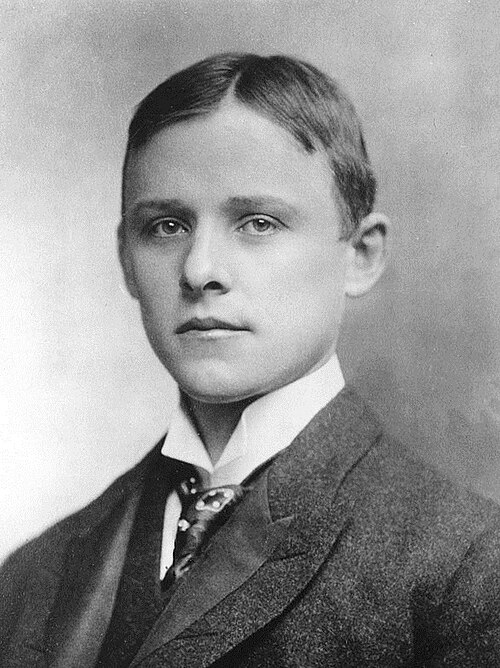
\includegraphics[width=\linewidth]{images/book3/hall.jpg}
\end{minipage}\hspace{0.02\linewidth}%
\begin{minipage}[t]{0.18\linewidth}
\vspace{0pt}
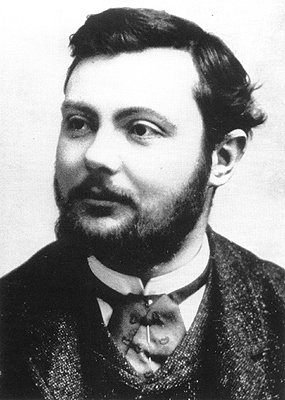
\includegraphics[width=\linewidth]{images/book3/heroult.jpg}
\end{minipage}\hfill
\begin{minipage}[t]{0.58\linewidth}
\vspace{0pt}
1886 年，年仅二十二或二十三岁的查尔斯·马丁·霍尔与
保罗·埃鲁在大西洋两岸各自独立地发现，氧化铝
可溶于熔融冰晶石，并可在其中\omterm{def:b2:batteries-electrolysis:electrolysis}{电解}。铝在此之前
是用钠还原其氯化物制得的贵金属，
大规模发电成为可能后，它成了最便宜的轻金属。
（肖像：霍尔，约 1880 年代，作者不详，公有领域；埃鲁，
公有领域；维基共享资源。）
\end{minipage}
\end{history}

\paragraph{钠。}钠不能从水中沉积出来，因为钠会还原水。
工业上通过\omterm{def:b2:batteries-electrolysis:electrolysis}{电解}熔融氯化钠制得，其熔点
借加入的盐而降低（即\omterm{def:b2:solid-liquid-diagrams:eutectic}{低共熔混合物}，见\cref{ch:b2:solid-liquid-diagrams}），
同时得到氯气作为副产物。在 \qty{1100}{K} 时，$\Delta_f G^\circ(\ce{NaCl}, \text{l}) =
\qty{-310.7}{kJ/mol}$，最小电压为 \qty{3.22}{V}。
% ledger: janafG:NaCl.1100

\section{练习}

\begin{exercise}[$\star$]\label{exo:b2:batteries-electrolysis:1}
根据锌在酸中的图，读出单独的锌以及与铜接触的锌的\omterm{def:b2:batteries-electrolysis:mixed-potential}{混合电势}及电流
（模型单位），并说明哪一种溶解
得更快。
\end{exercise}

\begin{exercise}[$\star$]\label{exo:b2:batteries-electrolysis:2}
以 \qty{500}{A} 的电流通电一小时，
\omterm{def:b2:batteries-electrolysis:faradaic-efficiency}{法拉第效率}为 100~\%，沉积出的锌的质量为多少？
\end{exercise}

\begin{exercise}[$\star$]\label{exo:b2:batteries-electrolysis:3}
根据本章给出的生成\omterm{def:b2:reaction-free-energy:gibbs-energy}{吉布斯自由能}，计算铅酸\omterm{def:b2:batteries-electrolysis:battery}{蓄电池}的标准电压，
并求
\qty{12}{V} 汽车电池中所含的单体电池数。
\end{exercise}

\begin{exercise}[$\star$]\label{exo:b2:batteries-electrolysis:4}
一克锂若全部氧化为
\ce{Li+}，能输出多少安时的电荷？
\end{exercise}

\begin{exercise}[$\star\star$]\label{exo:b2:batteries-electrolysis:5}
某铜精炼\omterm{def:b2:batteries-electrolysis:electrolysis}{电解槽}以 \qty{200}{A} 的电流通电 \qty{24}{h}，
沉积出 \qty{5.50}{kg} 铜。求其\omterm{def:b2:batteries-electrolysis:faradaic-efficiency}{法拉第效率}。
\end{exercise}

\begin{exercise}[$\star\star$]\label{exo:b2:batteries-electrolysis:6}
某锌\omterm{def:b2:batteries-electrolysis:electrolysis}{电解}提取槽在 \qty{3.3}{V} 下工作，\omterm{def:b2:batteries-electrolysis:faradaic-efficiency}{法拉第效率}为
90~\%（练习数据）。计算每千克锌所耗的电能。
\end{exercise}

\begin{exercise}[$\star\star$]\label{exo:b2:batteries-electrolysis:7}
某电池输出电压在 \qty{0.10}{A} 时为 \qty{1.55}{V}，在 \qty{0.60}{A} 时为 \qty{1.40}{V}。
假设\omterm{def:b2:current-potential-curves:overpotential}{过电势}可以忽略，求其内阻及
无电流时的电压。
\end{exercise}

\begin{exercise}[$\star\star$]\label{exo:b2:batteries-electrolysis:8}
在隔膜\omterm{def:b2:batteries-electrolysis:electrolysis}{电解槽}中\omterm{def:b2:batteries-electrolysis:electrolysis}{电解}食盐水。写出电极反应，
计算最小电压，并说明为何必须将两种产物
分开。
\end{exercise}

\begin{exercise}[$\star\star$]\label{exo:b2:batteries-electrolysis:9}
计算熔融氯化钠在
\qty{1100}{K} 下\omterm{def:b2:batteries-electrolysis:electrolysis}{电解}的最小电压，以及每千克钠所需的最小能量。
\end{exercise}

\begin{exercise}[$\star\star\star$]\label{exo:b2:batteries-electrolysis:10}
利用\omterm{def:b2:current-potential-curves:ie-curve}{电流–电势曲线}，解释为何可以在酸性
镀液中于锌阴极上镀锌，并预测铂阴极
在镀覆开始时会发生什么。
\end{exercise}

\begin{exercise}[$\star\star\star$]\label{exo:b2:batteries-electrolysis:11}
由 \qty{1100}{K} 和 \qty{1300}{K} 时的 $\Delta_f G^\circ$（$\ce{Al2O3}$：$-1328.3$ 和
$-1262.3$；$\ce{CO2}$：$-396.0$ 和 $-396.2$ \unit{kJ/mol}），计算
霍尔–埃鲁\omterm{def:b2:batteries-electrolysis:electrolysis}{电解槽}在 \qty{1250}{K} 时的最小电压，
并与释放氧气的惰性阳极相比较。
\end{exercise}

\begin{exercise}[$\star\star\star$]\label{exo:b2:batteries-electrolysis:12}
通过在 \qty{1.80}{V} 下\omterm{def:b2:batteries-electrolysis:electrolysis}{电解}水储存电能，
再在 \qty{0.70}{V} 下于\omterm{def:b2:batteries-electrolysis:fuel-cell}{燃料电池}中回收，二者的\omterm{def:b2:batteries-electrolysis:faradaic-efficiency}{法拉第效率}均为 100~\%。计算
往返效率，并说明能量的去向。
\end{exercise}

\section{问题：一吨铝}

\begin{problem}[{周末问题——霍尔–埃鲁电解槽的反应
及其最小电压，制备一吨铝所需的电荷与时间，
所用的能量以及烧掉的碳}]
\label{pb:b2:batteries-electrolysis:1}
数据：JANAF 在 \qty{1100}{K} 和 \qty{1300}{K} 下的生成\omterm{def:b2:reaction-free-energy:gibbs-energy}{吉布斯自由能}
（\unit{kJ/mol}）：\ce{Al2O3} $-1328.3$，$-1262.3$；\ce{CO2} $-396.0$，$-396.2$。\omterm{def:b2:batteries-electrolysis:electrolysis}{电解槽}
（练习数据）：电流 \qty{300}{kA}，电压 \qty{4.1}{V}，\omterm{def:b2:batteries-electrolysis:faradaic-efficiency}{法拉第效率}
94~\%，槽温接近 \qty{1250}{K}。摩尔质量（\unit{g/mol}）：Al 26.982，C 12.011，
O 15.999。将铝由 \qty{298}{K} 加热至熔点，使其成为液态，
所需热量为 \qty{28.69}{kJ/mol}。
% ledger: janafG:Al2O3.1100, janafG:Al2O3.1300, janafG:CO2.1100, janafG:CO2.1300, aw:Al, aw:C, aw:O, hT:Al_l.933, const:F

\medskip
\noindent\textbf{第一部分——最小电压。}
\begin{enumerate}
  \item 给出反应物和生成物中铝、氧和碳的
        氧化数。
  \item 写出阴极和阳极的半反应，其中氧离子
        \ce{O^2-} 由熔融\omterm{def:b2:batteries-electrolysis:electrolysis}{电解}质携带。
  \item 写出总反应，并给出转移电子数 $n$。
  \item 内插求 \qty{1250}{K} 时 $\Delta_f G^\circ$（\ce{Al2O3} 和 \ce{CO2}）。
  \item 计算 \qty{1250}{K} 时的 $\Delta_r G^\circ$。
  \item 推出最小电压。
  \item 计算使用惰性阳极时的最小电压，
        反应为 \ce{2Al2O3 -> 4Al + 3O2}，并说明碳的作用。
\end{enumerate}

\medskip
\noindent\textbf{第二部分——电荷与时间。}
\begin{enumerate}[resume]
  \item 一吨铝中所含铝的物质的量是多少？
  \item 若\omterm{def:b2:batteries-electrolysis:faradaic-efficiency}{法拉第效率}为 100~\%，需要多少电荷？
  \item 实际通过的电荷是多少？
  \item 一个\omterm{def:b2:batteries-electrolysis:electrolysis}{电解槽}制备一吨铝需要多长时间？
  \item 一个\omterm{def:b2:batteries-electrolysis:electrolysis}{电解槽}每天能制得多少质量的铝？
  \item 推测损失的 6~\% 电荷去向何处。
\end{enumerate}

\medskip
\noindent\textbf{第三部分——能量。}
\begin{enumerate}[resume]
  \item 计算每吨铝所耗的电能。
  \item 以 \unit{kW.h} 每千克表示该电能。
  \item 在最小电压和 100~\% 效率下，计算
        每千克铝所需的最小能量。
  \item 其余的能量去了哪里？为何它并非
        全部被浪费？
  \item 计算一个\omterm{def:b2:batteries-electrolysis:electrolysis}{电解槽}的电功率。
  \item 计算重熔一千克废铝所需的热量，
        单位为 \unit{kW.h}，并进行比较。
  \item 热力学最小电压占工作电压的几分之几？
\end{enumerate}

\medskip
\noindent\textbf{第四部分——碳。}
\begin{enumerate}[resume]
  \item 按该方程式计算每吨铝所烧掉的
        碳的质量。
  \item 计算每吨铝的阳极所释放的二氧化碳的质量。
  \item 实际\omterm{def:b2:batteries-electrolysis:electrolysis}{电解槽}烧掉的碳比这更多。请给出两个原因。
  \item 以每千克铝计，表示阳极的 \ce{CO2} 释放量。
  \item 若改用惰性阳极，电压和所释放的
        气体会发生什么变化？
  \item 写出每千克铝所耗的电能。
\end{enumerate}
\end{problem}
